\chapter{Практика}
\label{ch:chap2}

\subsection*{Задание 1: вычисление интеграла свертки сигнала и импульсной характеристики}

Зададим гармонический сигнал и импульсную характеристику RC цепи. Выполним операцию свертки и получим выходной сигнал.

\begin{figure}[H]
    \centering
    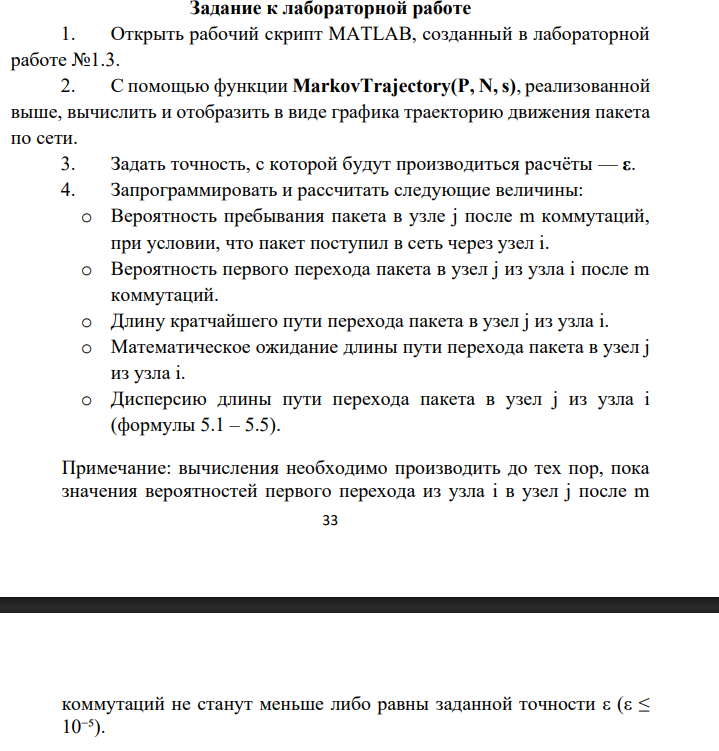
\includegraphics[width=1.0\textwidth]{task1.png}
    \caption{Задание 1}
\end{figure}

Можем заметить, что амплитуда кратно увеличилась, фаза тоже изменилась.

\subsection*{Задание 2: вычисление частотной характеристики RC цепи}

Вычислим АЧХ и ФЧХ RC цепи:

\begin{figure}[H]
    \centering
    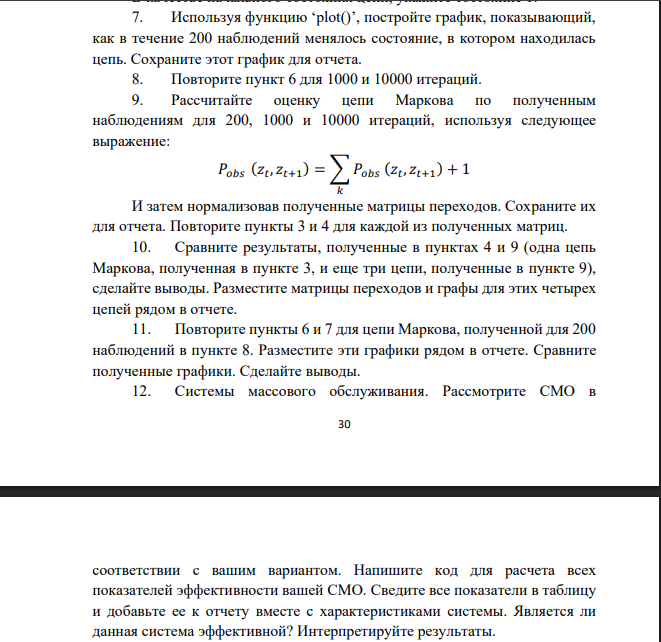
\includegraphics[width=1.0\textwidth]{task2.png}
    \caption{АЧХ и ФЧХ RC цепи}
\end{figure}

\subsection*{Задание 3: вычисление сигнала на выходе линейной цепи по частотной характеристике цепи}

Зная АЧХ и ФЧХ цепи, мы можем вычислить значение выходного сигнала. Наш сигнал имеет частоту 2000 Гц. Если посмотреть на график
АЧХ и ФЧХ, то этому значению соответствуют амплитуда 0.45В и фаза -1.9 рад. Выходной сигнал будет иметь вид $0.45cos(4000\pi+1.9)$. 

\begin{figure}[H]
    \centering
    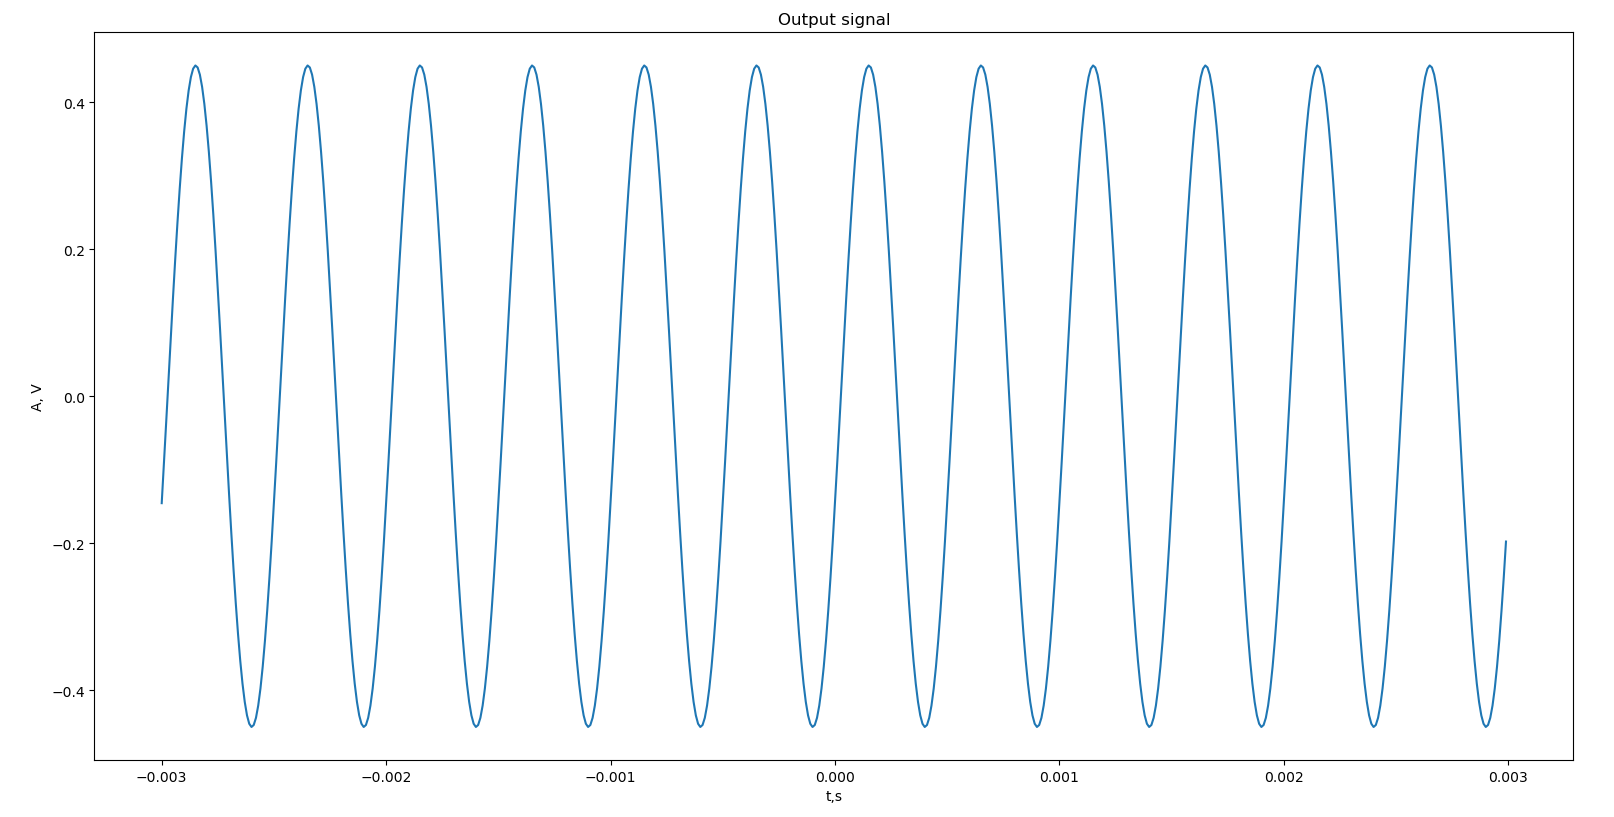
\includegraphics[width=1.0\textwidth]{out_sig.png}
    \caption{Выходной сигнал}
\end{figure}

Видим, что в выходном сигнале изменилась фаза и амплитуда, но форма сигнала осталась прежней.

\endinput